\cotefile{10}
\scanpage{42}
\mspage{\handwritten{10}}
\uline{pe de présentation finie, $H_j$ un $S_j$-préschéma de présentation finie à groupe d'\unsure{opérateurs|opératerus} $G_j$. Pour que $\mathbb{H}=H_j\handwritten{\times}_{S_j}S$ soit un $S$-préschéma en espaces homogènes sous $\deleted{\unsure{G|H}}\inserted{G=G_j\handwritten{\times}_{S_j}S}$ (resp. un fibré principal homogène sous $\unsure{G}\inserted{\deleted{\unsure{G=G_j\times_{S_j}S}}}$\unsure{)} pour la }\uuline{topologie fidèlement plate localement de présentation finie}\uline{, il faut et il suffit qu'il existe un indice $i\handwritten{\in}I$, $i\handwritten{\geq}j$, tel que $H_i=H_j\handwritten{\times}_{S_j}S_i$ soit un $S_i$-préschéma en espaces homogènes sous $\deleted{\unsure{G_i}}\inserted{G_i=G_j\handwritten{\times}_{S_j}S_i}$ (resp. un fibré principal homogène sous $G_i$).}

Compte tenu de (10.14) et de (EGA IV 8.8.2, 8.8.3 et 8.10.5) , \deleted{\unsure{l'exp|l'ex}} l'énoncé résulte de la propriété concernant les morphismes \deleted{\unsure{concernant|couvrant}}\inserted{couvrants} pour la topologie fppf rappelée en (10.0).

\figure{\begin{tikzpicture}[x=.5cm,y=.5cm]
\draw (0,11.6) .. controls (3.4,11.6) and (6.5,11.1) .. (5.1,10.2)
 .. controls (3.7,9.3) and (-1.8,7.2) .. (-.1,7.1)
 .. controls (1.9,7.0) and (4.1,7.6) .. (3.7,5.8)
 .. controls (3.5,4.8) and (2.1,3.8) .. (2.7,2.9)
 .. controls (3.4,1.9) and (5.0,1.1) .. (4.5,0);
\draw (2.45,11.7) .. controls (2.5,7.2) and (2.9,4.0) .. (3.75,.1);
\end{tikzpicture}}
% archive sheet number: 41
\scanpage{43}
\mspage{\handwritten{11}}
\uline{11.- Préschémas en groupes affines.}

\uline{\handwritten{11}.0.}- Notations : soient $S$ un préschéma, $X$ un $S$-préschéma, $f:X\handwritten{\to}S$ le morphisme structural; on pose $\handwritten{\unsure{\mathcal{A}|a}}(X)=f_{\handwritten{*}}(\handwritten{\mathcal{O}}_X)$.

\handwritten{\makebox[0pt][l]{\raisebox{-2ex}{\begin{tikzpicture}[x=1cm,y=1cm]\draw (0,.1) -- (.09,.1) -- (.09,-.07);\end{tikzpicture}}}}\uline{Lemme 11.1.- Soient $X$ et $Y$ deux $S$-préschémas quasi-compacts et quasi-séparés sur $S$, $f:X\handwritten{\to}S$ et $g:Y\handwritten{\to}S$ les morphismes structuraux. Alors l'homomorphisme canonique}
\[
\handwritten{\varphi}:\handwritten{\mathcal{A}}(X)\handwritten{\otimes}_{\handwritten{\mathcal{O}}_{\mathbb{S}}}\handwritten{\mathcal{A}}(Y)\handwritten{\longrightarrow}\handwritten{\mathcal{A}}(X\handwritten{\times}_S Y)
\]
% Curved pen mark below the tensor-base index.
\figure{\handwritten{\begin{tikzpicture}[x=1cm,y=1cm]\draw (0,.18) .. controls (.25,-.2) and (.8,-.18) .. (1.25,.22);\end{tikzpicture}}}
\margin{\handwritten{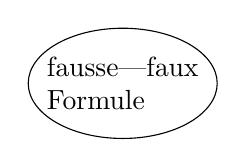
\begin{tikzpicture}[x=1cm,y=1cm]
\draw (0,0) ellipse (1.2 and .7);
\node[align=left] at (0,0) {\unsure{fausse|faux}\\Formule};
\end{tikzpicture}}}
\uline{est un isomorphisme dans chacun des cas suivants :}

\uline{a) $f$ et $g$ sont affines}

\uline{b) $f$ ou $g$ est plat et affine}

\uline{c) $g$ est plat et $f_{\handwritten{*}}(\handwritten{\mathcal{O}}_X)$ est un $\handwritten{\mathcal{O}}_S$-Module plat.}
% Curved pen mark below the star of f in c).
\figure{\handwritten{\begin{tikzpicture}[x=1cm,y=1cm]\draw (0,.15) .. controls (.15,-.16) and (.45,-.16) .. (.6,.16);\end{tikzpicture}}}
\margin{\handwritten{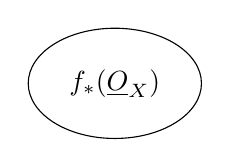
\begin{tikzpicture}[x=1cm,y=1cm]
\draw (0,0) ellipse (1.1 and .7);
\node at (0,0) {$f_*(\underline{O}_X)$};
\end{tikzpicture}}}

Dans le cas b), on peut supposer que c'est $g$ qui est plat et affine. Posons $S'=\operatorname{Spec}\handwritten{\mathcal{A}}(X\unsure{)}$ $Y'=Y\handwritten{\times}_S\mathbb{S}'$, $g'=g\handwritten{\times}_S S'$ et notons $v$ le morphisme $S'\handwritten{\to}S$. Alors $Y$ est quasi-compact et quasi-séparé sur $S$, et, ou bien $S'$est plat sur $S$ (cas c) d'après (EGA III (1.4.15.5)), ou bien $g$ est affine (cas a) et b)). Alors (EGA III 1.4.15 et IV 1.2.7 ou II 1.5.2), on a :
\[
g'_{\handwritten{*}}(\handwritten{\mathcal{O}}_{Y'})=v^{\handwritten{*}}g_{\handwritten{*}}(\handwritten{\mathcal{O}}_Y)=\handwritten{\mathcal{A}}(Y)\handwritten{\otimes}_{\handwritten{\mathcal{O}}_S}\handwritten{\mathcal{O}}_{S'}.
\]

D'après (EGA II 1.2.7), $f$ se factorise à travers $v$ au moyen \handwritten{\makebox[0pt][l]{\raisebox{2ex}{\begin{tikzpicture}[x=1cm,y=1cm]\draw (0,0) -- (.17,.09) -- (.43,-.05);\end{tikzpicture}}}}d'un morphisme $p:G\handwritten{\to}S'$, et on a : $X\handwritten{\times}_S Y=X\handwritten{\times}_{S'}Y'$ et $p_{\handwritten{*}}(\handwritten{\mathcal{O}}_X)=\handwritten{\mathcal{O}}_{S'}$. Puisque $v$ et $f$ sont quasi-compacts et quasi-séparés,\deleted{sur} il en est de même de $p$ (EGA IV 1.2.2 et 1.2.4)\handwritten{;} \handwritten{O}u bien $Y$ est plat sur $S$ (cas b) et c)) et alors $Y'$ est plat sur $S'$, ou bien $X$ est affine sur $S$ (cas a)), et alors $p$ est un isomorphisme. Dans le premier cas, on peut de nouveau appliquer (EGA III 1.4.15 et IV 1.2.7), et dans les deux cas, on trouve :
\[
\deleted{\unsure{p'_*|q'_*}}\ p'_{\handwritten{*}}(\handwritten{\mathcal{O}}_{X\handwritten{\times}_S Y})=g'^{\handwritten{*}}p_{\handwritten{*}}(\handwritten{\mathcal{O}}_X)=g'^{\handwritten{\unsure{*|\times}}}(\handwritten{\mathcal{O}}_{S'})=\handwritten{\mathcal{O}}_{Y'}\handwritten{,\ \text{ou }p'=p\times_{S'}Y'.}
\]

D'où :
\[
\handwritten{\mathcal{A}}(X\handwritten{\times}_S Y)=v_{\handwritten{*}}g'_{\handwritten{*}}p'_{\handwritten{*}}(\handwritten{\mathcal{O}}_{X\handwritten{\times}_S Y})=v_{\handwritten{*}}g'_{\handwritten{*}}(\handwritten{\mathcal{O}}_{\handwritten{Y}'})=v_{\handwritten{*}}(\handwritten{\mathcal{A}}(Y)\handwritten{\otimes}_{\handwritten{\mathcal{O}}_S}\handwritten{\mathcal{O}}_{S'})=\handwritten{\mathcal{A}}(Y)\handwritten{\otimes}_{\handwritten{\mathcal{O}}_S}\handwritten{\mathcal{A}}(X)
\]
d'après (EGA II 1.4.7).

\uline{Corollaire 11\handwritten{.}2.- On définit un foncteur $X\handwritten{\rightsquigarrow}\operatorname{Spec}\handwritten{\mathcal{A}}(X)$ de la sous-catégorie pleine de $\operatorname{Sch}_{/S}$ des $X$-préschémas plats quasi-compacts et quasi-séparés sur $S$ tels que $\handwritten{\mathcal{A}}(X)$ soit un $\handwritten{\mathcal{O}}_S$-Module plat , dans celle des $S$-préschémas plats et affines sur $S$ . Ce foncteur commute aux produits finis, donc transforme $S$-groupes en $S$-groupes.}
% archive sheet number: 42
\scanpage{44}
\mspage{\handwritten{12}}
\uline{Définition 11.3.}- Etant donné un $S$-groupe $G$ plat, quasi-compact et quasi-séparé sur $S$, tel que $\handwritten{\unsure{\mathcal{A}|a}}(G)$ soit plat sur $\handwritten{\mathcal{O}}_S$, nous noterons $G_{\mathrm{af}}$ , et nous appellerons \uline{enveloppe affine} de $G$ le $S$-groupe $G_{\mathrm{af}}=\operatorname{Spec}\handwritten{\mathcal{A}}(G)$.
\margin{\deleted{\handwritten{\unsure{vu}}}}

\uline{11.4.}- Etant donnés deux $\handwritten{\mathcal{O}}_S$-Modules $\handwritten{\mathcal{E}}$ et $\handwritten{\mathcal{F}}$ quasi-cohérents, notons $\handwritten{\mathcal{H}om}_S(\handwritten{\mathbb{V}}(\handwritten{\mathcal{F}}),\handwritten{\mathbb{V}}(\handwritten{\mathcal{E}}))$ le $S$-foncteur des morphismes de $S$-foncteurs de $\handwritten{\mathbb{V}}(\handwritten{\mathcal{F}})$ dans $\handwritten{\mathbb{V}}(\handwritten{\mathcal{E}})$, et $\handwritten{\mathcal{H}om}_{\handwritten{\mathcal{O}}_S}(\handwritten{\mathbb{V}}(\handwritten{\mathcal{F}}),\handwritten{\mathbb{V}}(\handwritten{\mathcal{E}}))$ le sous-$S$-foncteur de $\handwritten{\mathcal{H}om}_S(\handwritten{\mathbb{V}}(\handwritten{\mathcal{F}}),\handwritten{\mathbb{V}}(\handwritten{\mathcal{E}}))$ formé des $\handwritten{\mathcal{O}}_S$- homomorphismes de $\handwritten{\mathcal{O}}_S$-foncteurs en modules (cf. \deleted{Exp.} I). Alors $\handwritten{\mathcal{H}om}_{\handwritten{\mathcal{O}}_S}(\handwritten{\mathbb{V}}(\handwritten{\mathcal{F}}),\handwritten{\mathbb{V}}(\handwritten{\mathcal{E}}))(T)$ est en correspondance bi\deleted{n}\inserted{\handwritten{un}}ivoque canonique avec $\deleted{\unsure{\operatorname{Hom}}}\operatorname{Hom}_{\handwritten{\mathcal{O}}_{S\deleted{\unsure{T}}}\text{-}\mathrm{Mod.}}(\handwritten{\mathcal{E}\otimes}_{\handwritten{\mathcal{O}}_S}\handwritten{\mathcal{O}}_T,\deleted{\unsure{(}}\handwritten{\mathcal{F}\otimes}_{\handwritten{\mathcal{O}}_S}\handwritten{\mathcal{O}}_T\deleted{\unsure{)}}$,
\inserted{\handwritten{$\text{i.e.}\quad \mathcal{H}om_{\underline{O}_S}(\mathbb{V}(\mathcal{F}),\mathbb{V}(\mathcal{E}))\simeq\mathcal{H}om_{\underline{O}_S}(\mathbb{W}(\mathcal{E}),\mathbb{W}(\mathcal{F})).$}}
\margin{\handwritten{\unsure{vu}}}

Soit $X$ un $S$-préschéma. Alors l'ensemble des morphismes de $S$-foncteurs de $X$ dans $\handwritten{\mathcal{H}om}_S(\deleted{\handwritten{\unsure{\mathbb{V}|W}}}\handwritten{\mathbb{V}}(\handwritten{\mathcal{F}}),\handwritten{\mathbb{V}}(\handwritten{\mathcal{E}}))$ est en correspondance bi\inserted{\handwritten{un}}nivoque avec $\operatorname{Hom}_S(X\handwritten{\times}_S\handwritten{\mathbb{V}}(\handwritten{\mathcal{F}}),\handwritten{\mathbb{V}}(\handwritten{\mathcal{E}}))$, donc l'ensemble des morphismes de $S$-foncteurs de $X$ dans $\handwritten{\mathcal{H}om}_{\handwritten{\mathcal{O}}_S}(\handwritten{\mathbb{V}}(\handwritten{\mathcal{F}}),\handwritten{\mathbb{V}}(\handwritten{\mathcal{E}}))$ est en correspondance biunivoque avec un sous-ensemble de $\operatorname{Hom}_S(X\handwritten{\times}_S\handwritten{\mathbb{V}}(\handwritten{\mathcal{F}}),\handwritten{\mathbb{V}}(\handwritten{\mathcal{E}}))=\operatorname{Hom}_{\handwritten{\mathcal{O}}_S\text{-}\unsure{\mathrm{Mod.}|\mathrm{Mod;}}}(\handwritten{\mathcal{E}},\handwritten{\mathcal{A}}(X\handwritten{\times}_S\handwritten{\mathbb{V}}(\handwritten{\mathcal{F}})))$ (EGA II 1.7.13).

\uline{Proposition 11.5.- Soient $X$ un $S$-préschéma quasi-compact quasi-séparé sur $S$, $f:X\handwritten{\to}S$ le morphisme structural, $\handwritten{\mathcal{E}}$ et $\handwritten{\mathcal{F}}$ deux $\handwritten{\mathcal{O}}_S$-Modules quasi-cohérents. On suppose vérifiée\deleted{s} l'une des deux conditions suivantes :}

\uline{a) $f$ est affine}

\uline{b) $\handwritten{\mathcal{F}}$ est plat sur $\handwritten{\mathcal{O}}_S$.}

\uline{Alors :}

\margin{\handwritten{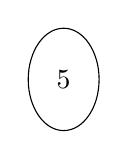
\begin{tikzpicture}\draw (0,0) ellipse (.45 and .65);\node at (0,0) {5};\end{tikzpicture}}}
\uline{i) l'homomorphisme canonique $\handwritten{\varphi:\mathcal{A}}(X)\handwritten{\otimes}_{\handwritten{\mathcal{O}}_S}\handwritten{\mathbb{S}}(\handwritten{\mathcal{F}})\handwritten{\longrightarrow\mathcal{A}}(X\handwritten{\times}_S\handwritten{\mathbb{V}}(\handwritten{\mathcal{F}}))$ est un isomorphisme (où $\handwritten{\mathbb{S}}(\handwritten{\mathcal{F}})$ désigne l'Algèbre symétrique de $\handwritten{\mathcal{F}}$).}

\uline{ii) l'ensemble des morphismes de $S$-foncteurs de $X$ dans $\handwritten{\mathcal{H}om}_{\handwritten{\mathcal{O}}_S}(\handwritten{\mathbb{V}}(\handwritten{\mathcal{F}}),\handwritten{\mathbb{V}}(\handwritten{\mathcal{E}}))$ est en correspondance biunivoque avec $\operatorname{Hom}_{\handwritten{\mathcal{O}}_S\text{-}\mathrm{Mod.}}(\handwritten{\mathcal{E}}\ ,\ \handwritten{\mathcal{A}}(X)\handwritten{\otimes\mathcal{F}})$.}

Pour montrer i), d'après (11.1, a) et b)), il suffit de montrer que si $\handwritten{\mathcal{F}}$ est plat sur $\handwritten{\mathcal{O}}_{\mathbb{S}}$, \deleted{\unsure{il en est de même de} $\handwritten{\mathbb{S}}(\handwritten{\mathcal{F}})$} alors $\handwritten{\mathbb{V}}(\handwritten{\mathcal{F}})$ est plat sur $S$. D'après (EGA III 1.4.15.5),
% archive sheet number: 43
\scanpage{45}
\mspage{\handwritten{13}}
il suffit de voir que si $\handwritten{\mathcal{F}}$ est plat sur $\handwritten{\mathcal{O}}_S$, \inserted{il en est de même de $\handwritten{\mathbb{S}\mathcal{F}}$} ce qui \deleted{résulte des définitions (EGA II 1.7.1), compte tenu d'}\inserted{\handwritten{est un corollaire d'}}un resultat dû à Daniel LAZARD, suivant lequel tout\deleted{e limite inductive de modules plats est un} module plat\deleted{.} \inserted{\handwritten{sur un anneau est une limite inductive filtrante de modules libres de type fini.}}

\deleted{Remarquons de plus que $\handwritten{\unsure{\mathcal{A}|a}}(X)\handwritten{\otimes}_{\handwritten{\mathcal{O}}_S}\handwritten{\mathbb{S}\mathcal{F}}=\handwritten{\mathbb{S}}(\handwritten{\mathcal{A}}(X)\handwritten{\otimes}_{\handwritten{\mathcal{O}}_S}\handwritten{\mathcal{F}})$ d'après (EGA II 1.1.2), ce qui montre que l'homomorphisme canonique $\handwritten{\mathcal{A}}(X)\handwritten{\otimes}_{\handwritten{\mathcal{O}}_S}\handwritten{\mathcal{F}\longrightarrow}\deleted{\handwritten{\unsure{\mathbb{S}|(}}}\handwritten{\mathcal{A}}(X)\handwritten{\otimes}_{\handwritten{\mathcal{O}}_S}\handwritten{\mathbb{S}\mathcal{F}}\deleted{\unsure{)}}$ est injectif.}

Montrons maintenant ii). Soit $\handwritten{\alpha}$ un morphisme de $S$-foncteurs de $X$ dans $\handwritten{\mathcal{H}om}_{\handwritten{\mathcal{O}}_S}(\handwritten{\mathbb{V}}(\handwritten{\mathcal{F}}),\handwritten{\mathbb{V}}(\handwritten{\mathcal{E}}))$; il lui correspond un homomorphisme $\handwritten{\rho}$ de $\handwritten{\mathcal{O}}_S$-Modules de $\handwritten{\mathcal{E}}$ dans $\handwritten{\mathcal{A}}(X\handwritten{\times}_S\handwritten{\mathbb{V}}(\handwritten{\mathcal{F}}))=\handwritten{\mathcal{A}}(X)\handwritten{\otimes}_{\handwritten{\mathcal{O}}_S}\handwritten{\mathbb{S}}(\handwritten{\mathcal{F}})$ tel que si $\handwritten{\rho}$ est une $S$-section de $X$, l'homomorphisme
\[
(\handwritten{\mathcal{A}(\eta)\otimes}\operatorname{id}_{\handwritten{\mathbb{S}\mathcal{F}}})\handwritten{\circ\rho}:\handwritten{\mathcal{E}\longrightarrow\mathcal{O}}_S\handwritten{\otimes}_{\handwritten{\mathcal{O}}_S}\handwritten{\mathbb{S}\mathcal{F}=\mathbb{S}\mathcal{F}}
\]
corresponde à $\handwritten{\alpha(\eta)}$. Mais puisque $\handwritten{\alpha(\eta)\in}\deleted{\handwritten{\unsure{\mathcal{E}|\mathcal{H}om}}}\handwritten{\mathcal{H}om}_{\handwritten{\mathcal{O}}_S}(\handwritten{\mathbb{V}}(\handwritten{\mathcal{F}}),\handwritten{\mathbb{V}}(\handwritten{\mathcal{E}}))(S)$, $\handwritten{\mathcal{A}(\eta)\otimes}\operatorname{id}_{\handwritten{\mathbb{S}\mathcal{F}}}$ se factorise à travers l'homomorphisme canonique injectif $\handwritten{\mathcal{F}\to\mathbb{S}\mathcal{F}}$. On a donc, pour chaque $S$-section $\handwritten{\eta}$ de $X$\handwritten{,}un diagramme commutatif :
\margin{\handwritten{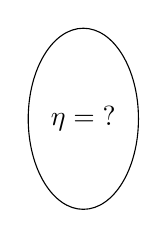
\begin{tikzpicture}
\draw (0,0) ellipse (.7 and 1.15);
\node at (0,0) {$\eta={?}$};
\end{tikzpicture}}}
\diagram{\handwritten{\begin{tikzcd}[ampersand replacement=\&]
\mathcal{E}\arrow[r,"\rho"]\arrow[d] \& \mathcal{A}(X)\otimes\mathbb{S}\mathcal{F}\arrow[d]\arrow[dl,"\mathcal{A}(\eta)\otimes\operatorname{id}"']\\
\mathbb{S}\mathcal{F} \& \mathcal{F}\arrow[l]
\end{tikzcd}}}
\handwritten{,}

ce qui montre que $\handwritten{\rho}$ se factorise à travers l'homomorphisme canonique injectif $\handwritten{\mathcal{A}}(X)\handwritten{\otimes}_{\handwritten{\mathcal{O}}_S}\handwritten{\mathcal{F}\longrightarrow\mathcal{A}}(X)\handwritten{\otimes}_{\handwritten{\mathcal{O}}_S}\handwritten{\mathbb{S}\mathcal{F}}$ , donc $\handwritten{\rho}$ peut être considéré comme un homomorphisme de $\handwritten{\mathcal{O}}_S$-Modules de $\handwritten{\mathcal{E}}$ dans $\handwritten{\mathcal{A}}(X)\handwritten{\otimes}_{\handwritten{\mathcal{O}}_S}\handwritten{\mathcal{F}}$ .

Réciproquement, soit $\handwritten{\rho\in}\operatorname{Hom}_{\handwritten{\mathcal{O}}_S\text{-}\mathrm{Mod.}}(\handwritten{\mathcal{E}}\ ,\ \handwritten{\mathcal{A}}(X)\handwritten{\otimes}_{\handwritten{\mathcal{O}}_S}\handwritten{\mathcal{F}})\handwritten{\subset}\operatorname{Hom}_{\handwritten{\mathcal{O}}_S\text{-}\mathrm{Mod}}(\handwritten{\mathcal{E}}\ ,\ \handwritten{\mathcal{A}}(X\handwritten{\times}_S\handwritten{\mathbb{V}}(\handwritten{\mathcal{F}})))$ ; il lui correspond un morphisme $\handwritten{\alpha}$ de $X$ dans $\handwritten{\mathcal{H}om}_{\mathbb{S}}(\handwritten{\mathbb{V}}(\handwritten{\mathcal{F}}),\handwritten{\mathbb{V}}(\handwritten{\mathcal{E}}))$ . Pour tout $S$-préschéma $T$ et toute $T$-section $\handwritten{\eta}$ de $X\handwritten{\times}_S T$ , $\handwritten{\alpha(\eta)}$ correspond à $\handwritten{\mathcal{A}(\eta)\otimes}\operatorname{id}_{\handwritten{\mathbb{S}\mathcal{F}\otimes\mathcal{O}}_T}$ , homomorphisme de $\handwritten{\mathcal{E}\otimes}_{\handwritten{\mathcal{O}}_S}\handwritten{\mathcal{O}}_T$ dans $\handwritten{\mathcal{F}\otimes}_{\handwritten{\mathcal{O}}_S}\handwritten{\mathcal{O}}_T$ , donc $\handwritten{\unsure{\alpha|d}(\eta)\in\mathcal{H}om}_{\handwritten{\mathcal{O}}_S}(\handwritten{\mathbb{V}}(\handwritten{\mathcal{F}}),\handwritten{\mathbb{V}}(\handwritten{\mathcal{E}}))(T)$, ce qui montre que $\handwritten{\alpha}$ est un morphisme de $X$ dans $\handwritten{\mathcal{H}om}_{\handwritten{\mathcal{O}}_S}(\handwritten{\mathbb{V}}(\handwritten{\mathcal{E}}),\handwritten{\mathbb{V}}(\handwritten{\mathcal{F}}))$, ce qui prouve ii).

\deleted{\unsure{Corollaire 11.6.- Soit} $G$ un $S$-groupe plat, quasi-compact et quasi-séparé sur $S$, \unsure{tel que} $\handwritten{\mathcal{A}}(G)$ soit un $\handwritten{\mathcal{O}}_S$-module plat, \deleted{\unsure{et}} $\handwritten{\mathcal{E}}$ un $\handwritten{\mathcal{O}}_S$-Module quasi-cohérent et plat. Alors l'ensemble des applications linéaires}
% archive sheet number: 44
\scanpage{46}
\mspage{\handwritten{14}}
\uline{11.6.}- Soient $G$ un $S$-groupe plat quasi-compact et quasi-séparé sur $S$ tel que $\handwritten{\unsure{\mathcal{A}|a}}(G)$ soit un $\handwritten{\mathcal{O}}_S$-Module plat $\handwritten{\mathcal{A}}$, et $\handwritten{\mathcal{E}}$ un $\handwritten{\mathcal{O}}_S$-Module quasi-cohérent et plat. \deleted{Nous dirons qu'}\inserted{\handwritten{Notons qu'}}un morphisme de $S$-foncteurs de $G$ dans $\inserted{\handwritten{\operatorname{End}_{\mathcal{O}_{\mathbb{S}}}(\unsure{\mathbb{W}|W}(\mathcal{E}))}}\deleted{\handwritten{\unsure{\mathcal{H}om_{\mathcal{O}_S}(\mathcal{E},\mathcal{E})}}}\handwritten{\simeq\mathcal{H}om}_{\handwritten{\mathcal{O}}_S}(\handwritten{\mathbb{V}}(\handwritten{\mathcal{E}}),\handwritten{\mathbb{V}}(\handwritten{\mathcal{E}}))$ définit une \uline{opération} de $G$ sur $\handwritten{\mathcal{E}}$\handwritten{,} si \inserted{\handwritten{et seulement si}} le morphisme correspondant $\handwritten{\theta}:G\handwritten{\times}_S\handwritten{\mathbb{V}}(\handwritten{\mathcal{E}})\handwritten{\longrightarrow\mathbb{V}}(\handwritten{\mathcal{E}})$ vérifie les deux conditions suivantes :

$1^\circ)$ si $\handwritten{\mu}:G\handwritten{\times}_S G\handwritten{\longrightarrow}G$ désigne le morphisme structural, le diagramme
\diagram{\begin{tikzcd}[ampersand replacement=\&]
G\handwritten{\times}_S G\handwritten{\times}_S\handwritten{\mathbb{V}}(\handwritten{\mathcal{E}})
 \arrow[r,"\operatorname{id}_G\handwritten{\times\theta}"]\arrow[d,"\handwritten{\mu\times}\operatorname{id}_{\handwritten{\mathbb{V}(\mathcal{E})}}"']
\& G\handwritten{\times}_S\handwritten{\mathbb{V}}(\handwritten{\mathcal{E}})\arrow[d,"\handwritten{\theta}"]\\
G\handwritten{\times}_S\deleted{\unsure{X}}\handwritten{\mathbb{V}}(\handwritten{\mathcal{E}})\arrow[r,"\handwritten{\theta}"']
\& \handwritten{\mathbb{V}}(\handwritten{\mathcal{E}})
\end{tikzcd}}
\inserted{\figure{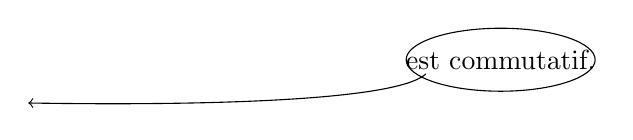
\begin{tikzpicture}[x=1cm,y=1cm]\handwritten{\draw (0,0) ellipse (1.2 and .4);\draw[->] (-.95,-.18) .. controls (-1.45,-.65) and (-5.8,-.55) .. (-6,-.55);}\node at (0,0) {est commutatif.};\end{tikzpicture}}}

$2^\circ)$ si $\handwritten{\varepsilon}:S\handwritten{\to}G$ est la section unité de $G$, le diagramme
\diagram{\begin{tikzcd}[ampersand replacement=\&]
S\handwritten{\times}_S\handwritten{\mathbb{V}}(\handwritten{\mathcal{E}})
 \arrow[rr,"\handwritten{\varepsilon\times}\operatorname{id}_{\handwritten{\mathbb{V}(\mathcal{E})}}"]
\& \& G\handwritten{\times}_S\handwritten{\mathbb{V}}(\handwritten{\mathcal{E}})\arrow[dl,"\handwritten{\theta}"]\\
\& \handwritten{\mathbb{V}}(\handwritten{\mathcal{E}})\arrow[ul,"\handwritten{\sim}"] \&
\end{tikzcd}}
\inserted{\figure{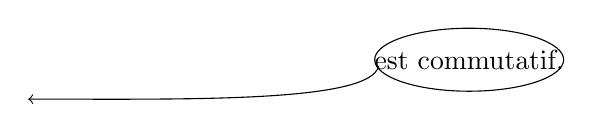
\begin{tikzpicture}[x=1cm,y=1cm]\handwritten{\draw (0,0) ellipse (1.2 and .4);\draw[->] (-1.15,-.08) .. controls (-1.25,-.55) and (-3.6,-.5) .. (-5.6,-.5);}\node at (0,0) {est commutatif.};\end{tikzpicture}}}

Il revient\inserted{\handwritten{alors}} au même de dire que le morphisme $\handwritten{\rho}:\inserted{\handwritten{\mathcal{E}\longrightarrow}}\handwritten{\mathcal{A}}(G)\handwritten{\otimes}_{\handwritten{\mathcal{O}}_{\mathbb{S}}}\handwritten{\mathcal{E}}$ déduit de $\handwritten{\theta}$ vérifie les deux axiomes suivants :
\margin{\handwritten{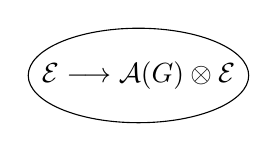
\begin{tikzpicture}
\draw (0,0) ellipse (1.4 and .6);
\node at (0,0) {$\mathcal{E}\longrightarrow\mathcal{A}(G)\otimes\mathcal{E}$};
\end{tikzpicture}}}

(CM1) Si $\handwritten{\Delta}:\handwritten{\mathcal{A}\longrightarrow\mathcal{A}\otimes\mathcal{A}}=\handwritten{\mathcal{A}}(G\handwritten{\times}_S G)$ est l'homomorphisme $\handwritten{\mathcal{A}(\theta)}$, le diagramme
\diagram{\handwritten{\begin{tikzcd}[ampersand replacement=\&]
\mathcal{A}\otimes\mathcal{A}\otimes\mathcal{A}
\& \mathcal{A}\otimes\mathcal{E}\arrow[l,"\operatorname{id}_{\mathcal{A}}\otimes\rho"']\\
\mathcal{A}\otimes\mathcal{E}\arrow[u,"\Delta\otimes\operatorname{id}_{\mathcal{E}}"]
\& \mathcal{A}\arrow[u,"\rho"']\arrow[l,"\rho"]
\end{tikzcd}}}
\inserted{\figure{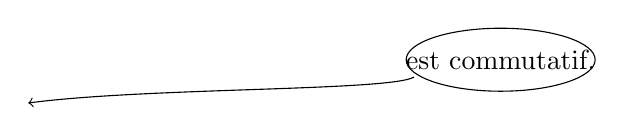
\begin{tikzpicture}[x=1cm,y=1cm]\handwritten{\draw (0,0) ellipse (1.2 and .4);\draw[->] (-1.1,-.22) .. controls (-1.4,-.4) and (-4.5,-.35) .. (-6,-.55);}\node at (0,0) {est commutatif.};\end{tikzpicture}}}

(CM2) Si $\handwritten{\eta}:\handwritten{\mathcal{A}\to\mathcal{O}}_S$ est l'homomorphisme $\handwritten{\mathcal{A}(\varepsilon)}$, le diagramme
\diagram{\handwritten{\begin{tikzcd}[ampersand replacement=\&]
\mathcal{O}_S\otimes\mathcal{E}
\& \& \mathcal{A}\otimes\mathcal{E}\arrow[ll,"\eta\otimes\operatorname{id}_{\mathcal{E}}"']\\
\& \mathcal{E}\arrow[ul,"\sim"]\arrow[ur,"\rho"']\&
\end{tikzcd}}}
\inserted{\figure{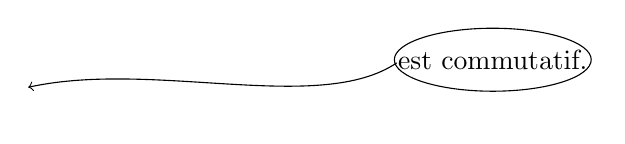
\begin{tikzpicture}[x=1cm,y=1cm]\handwritten{\draw (0,0) ellipse (1.25 and .4);\draw[->] (-1.22,-.04) .. controls (-2.2,-.7) and (-4.3,.0) .. (-5.9,-.35);}\node at (0,0) {est commutatif.};\end{tikzpicture}}}

Il revient au même de dire que le morphisme $\handwritten{\theta}_{\mathrm{af}}:G_{\mathrm{af}}\handwritten{\times}_S\handwritten{\mathbb{V}}(\handwritten{\mathcal{E}})\handwritten{\longrightarrow\mathbb{V}}(\handwritten{\mathcal{E}})$ correspondant à $\handwritten{\rho}$ définit une opération de $G_{\mathrm{af}}$ sur $\handwritten{\mathcal{E}}$ \deleted{\handwritten{\unsure{(Exp. I)}}} \inserted{\handwritten{(\unsure{compar|comparer} I \unsure{4|9}.2)}}.

Par conséquent, il y a correspondance biunivoque entre opérations de $G$ sur $\handwritten{\mathcal{E}}$ et opérations de $G_{\mathrm{af}}$ sur $\handwritten{\mathcal{E}}$.

\uline{\handwritten{L}emme} 11.7.- Soient $G$ un $S$-groupe quasi-compact et quasi-séparé sur $S$\handwritten{,}\inserted{\handwritten{plat et}} tel que $\handwritten{\mathcal{A}}(G)$ soit
% archive sheet number: 45
\scanpage{47}
\mspage{\handwritten{15}}
un $\handwritten{\mathcal{O}}_S$-Module plat $\handwritten{\unsure{\mathcal{A}|a}}$ , et $\handwritten{\mathcal{E}}$ un $\handwritten{\mathcal{O}}_S$-Module quasi-cohérent. On suppose soit que $G$ est affine\inserted{\handwritten{sur $S$}}, soit que \deleted{\unsure{G e}}t $\handwritten{\mathcal{E}}$ \deleted{son}\handwritten{soi}t plat\deleted{s} sur $S$. Soit $\handwritten{\rho:\mathcal{E}\to\mathcal{A}\otimes\mathcal{E}}$ un homomorphisme définissant une opération de $G$ sur $\handwritten{\mathcal{E}}$. Soit $\handwritten{\mathcal{E}}_{\unsure{o|0}}$ un sous-$\handwritten{\mathcal{O}}_S$-Module quasi-cohérent de $\handwritten{\mathcal{E}}$ tel que l'homomorphisme $\handwritten{\mathcal{E}}_o\handwritten{\longrightarrow\mathcal{A}\otimes\mathcal{E}}$ déduit de $\handwritten{\rho}$ se factorise à travers l'homomorphisme canonique \handwritten{(}injectif\inserted{\handwritten{, grâce au fait que $\mathcal{A}$ est plat !)}} $\handwritten{\mathcal{A}\otimes\mathcal{E}_o\longrightarrow\mathcal{A}\otimes\mathcal{E}}$ au moyen de l'homomorphisme $\handwritten{\rho_o:\mathcal{E}_o\longrightarrow\mathcal{A}\otimes\mathcal{E}_o}$. Alors $\handwritten{\rho_o}$ définit une opération de $G$ sur $\handwritten{\mathcal{E}_o}$\handwritten{(},\handwritten{\unsure{(}} qu'on appellera \uline{opération induite} sur $\handwritten{\mathcal{E}}_o$ par $\handwritten{\rho}$, et on dira que $\handwritten{\mathcal{E}}_o$ est \uline{stable} sous $\handwritten{\rho)}$.

Cela résulte immédiatement des définitions et de (11.\handwritten{6}). On remarquera cependant qu'en général l'application canonique $\handwritten{\mathbb{W}}(\handwritten{\mathcal{E}}_o)\handwritten{\longrightarrow\mathbb{W}}(\handwritten{\mathcal{E}})$ n'est pas injective.

\uline{Lemme 11.8.- Soient $G$ un $S$-groupe quasi-séparé et quasi-compact sur $S$ tel que $\handwritten{\mathcal{A}}(G)$ soit un $\handwritten{\mathcal{O}}_{\mathbb{S}}$-Module \deleted{\unsure{plat} $\handwritten{\mathcal{A}}$} libre $\handwritten{\mathcal{A}}$ de base $(\handwritten{\varphi}_i)$, $\handwritten{\mathcal{E}}$ un $\handwritten{\mathcal{O}}_S$-Module quasi-cohérent. On suppose soit que $G$ est affine\inserted{\handwritten{sur $S$}}, soit que $G$ et $\handwritten{\mathcal{E}}$ sont plats sur $S$. Soit $\handwritten{\rho:\mathcal{E}\to\mathcal{A}\otimes\mathcal{E}}$ un homomorphisme définissant une opération de $G$ sur $\handwritten{\mathcal{E}}$, et soit $x\handwritten{\in\Gamma}(S,\handwritten{\mathcal{E}})$. Posons $\handwritten{\rho}(x)=\handwritten{\sum\varphi}_i\handwritten{\otimes x}_i$, où les $x_i\handwritten{\in\Gamma}(S,\handwritten{\mathcal{E}})$ sont bien déterminés par cette relation). Alors le sous-module\inserted{\handwritten{$\mathcal{F}$}} de $\handwritten{\mathcal{E}}$ engendré par les $x_i$ est stable sous $\handwritten{\rho}$,\deleted{et contient $x$.}\inserted{quasi-cohérent} et de type fini sur $\handwritten{\mathcal{O}}_S$, et $x\handwritten{\in\Gamma}(S,\handwritten{\mathcal{F}})$.}
\figure{\handwritten{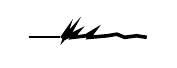
\begin{tikzpicture}[x=1cm,y=1cm]\draw[line width=.7pt] (0,0) -- (.4,0);\draw[line width=1.3pt] (.42,-.01) -- (.49,.09) -- (.46,0) -- (.55,.1) -- (.5,.01) -- (.62,.07) -- (.56,0) -- (.73,.02) -- (.83,.08) -- (.77,0) -- (1,.02) -- (1.12,.04) -- (1.22,0) -- (1.37,.02) -- (1.5,0);\end{tikzpicture}}}

\deleted{Soit $\handwritten{\mathcal{F}}$ le sous-module de $\handwritten{\mathcal{E}}$ engendré par les $x_i$.} \handwritten{I}l est clair que $\handwritten{\mathcal{F}}$ est quasi-cohérent et de type fini. L'axiome (CM1) montre que $\handwritten{\sum\Delta}(\handwritten{\varphi}_i)\handwritten{\otimes}x_i=\handwritten{\sum\varphi}_i\handwritten{\otimes\rho}(x_i)$ ; d'autre part, $\handwritten{\Delta(\varphi}_i\handwritten{)=\sum\varphi}_j\handwritten{\otimes}a_{ij}$ , d'où $\handwritten{\sum\varphi}_j\handwritten{\otimes}a_{ij}\handwritten{\otimes}x_i=\handwritten{\sum\varphi}_i\handwritten{\otimes\rho}(x_i)$, d'où, puisque les $\handwritten{\varphi}_i$ forment une base de $\handwritten{\mathcal{A}}$, $\handwritten{\rho}(x_i)=\handwritten{\sum}a_{ji}\handwritten{\otimes}x_{\handwritten{i}}$, où $a_{ji}\handwritten{\in\Gamma}(S,\handwritten{\mathcal{A}})$, ce qui montre que $\handwritten{\rho(\mathcal{F})\subset\mathcal{A}\otimes\mathcal{F}}$, donc $\handwritten{\mathcal{F}}$ est stable sous $\handwritten{\rho}$. Enfin l'axiome (CM2) montre que $x=\handwritten{\sum_i\eta}(\handwritten{\varphi}_i)x_i\handwritten{\in\Gamma}(S,\handwritten{\mathcal{F}})$.

\uline{Proposition 11.9.- Soit $G$ un $S$-groupe quasi-compact quasi-séparé sur $S$ tel que $\handwritten{\mathcal{A}}=\handwritten{\mathcal{A}}(G)$ devienne localement libre après extension fidèlement plate quasi-compacte de la base $S$ (ce qui est le cas\inserted{\handwritten{par exemple}} lorsque $G$ est un groupe réductif, comme nous\deleted{\unsure{l}} le verrons dans \deleted{l'exposé} \handwritten{$\overline{\underline{\mathrm{XXV}}}$}), et soit $\handwritten{\mathcal{E}}$ un $\handwritten{\mathcal{O}}_S$-\deleted{module}\handwritten{Module} quasi-cohérent . On suppose soit que $G$ est affine\inserted{\handwritten{sur $S$}}, soit que $G$ et $\handwritten{\mathcal{E}}$ sont plats sur $S$. Soit $\handwritten{\rho:\mathcal{E}\longrightarrow\mathcal{A}\otimes\mathcal{E}}$ un homomorphisme définissant une opération de $G$ sur $\handwritten{\mathcal{E}}$.}
% archive sheet number: 46
\scanpage{48}
\mspage{\handwritten{16}}
\uline{Alors, pour tout sous-$\handwritten{\mathcal{O}}_S$-Module quasi-cohérent $\handwritten{\mathcal{F}}$ de $\handwritten{\mathcal{E}}$ il existe un plus petit sous-$\handwritten{\mathcal{O}}_S$-Module quasi-cohérent $\handwritten{\widetilde{\mathcal{F}}}$ de $\handwritten{\mathcal{E}}$ contenant $\handwritten{\mathcal{F}}$ qui soit stable sous $\handwritten{\rho}$.}\inserted{\figure{\handwritten{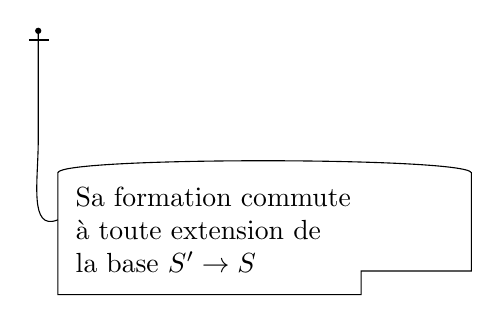
\begin{tikzpicture}[x=1cm,y=1cm]
\draw (.25,.1) .. controls (-.12,-.05) and (0,.6) .. (0,1.1) -- (0,2.5);
\fill (0,2.5) circle (.04);\draw[line width=.8pt] (-.12,2.38) -- (.14,2.38);
\draw (.25,.7) .. controls (.3,.9) and (5.4,.9) .. (5.5,.7) -- (5.5,-.55) -- (4.1,-.55) -- (4.1,-.85) -- (.25,-.85) -- cycle;
\node[align=left,anchor=west] at (.35,-.03) {Sa formation commute\\à toute extension de\\la base $S'\to S$};
\end{tikzpicture}}}}\uline{Lorsque $\handwritten{\mathcal{F}}$ est de type \deleted{\illegible{1}} fini, il en est de même de $\handwritten{\mathcal{F}}$.}

On se ramène aisément\inserted{\handwritten{par descente fidèlement plate}} au cas où $\handwritten{\unsure{\mathcal{A}|a}}$ est un $\handwritten{\mathcal{O}}_S$-Module libre, auquel cas la proposition est conséquence du lemme 11.8.

\uline{Corollaire 11.10.- \deleted{Soit}\inserted{Soient} $S$ un \deleted{pré} schéma \deleted{affine}\inserted{\handwritten{quasi-compact quasi-séparé}}, $G$ un $S$-groupe quasi-séparé\inserted{\handwritten{et}}quasicompact sur $S$ , tel que $\handwritten{\mathcal{A}}(G)$ devienne \deleted{\unsure{libre}} localement libre après extension fidèlement plate quasi-compacte de la base,$S$, et soit $\handwritten{\mathcal{E}}$ un $\handwritten{\mathcal{O}}_S$-Module quasi-cohérent. On suppose soit que $G$ est affine sur $S$\deleted{\unsure{.}}\handwritten{,}soit que $G$ et $\handwritten{\mathcal{E}}$ sont plats sur $S$\handwritten{.}\inserted{On se donne une opération de $G$ sur $\handwritten{\mathcal{E}}$\handwritten{.}} \handwritten{A}lors $\handwritten{\mathcal{E}}$ est limite inductive d'une famille filtrante croissante de sous- $\handwritten{\mathcal{O}}_S$-Modules quasi-cohérents de type fini de $\handwritten{\mathcal{E}}$ stables sous $\handwritten{G}$.}

C'est une conséquence immédiate de (11.9) car $\handwritten{\mathcal{E}}$ est \deleted{engendré par ses sections (EGA I 1.4.\unsure{1}) et car l'ensemble des sous-$\handwritten{\mathcal{O}}_S$-Modules quasi-cohérents de type fini de $\handwritten{\mathcal{E}}$ stables sous $G$ est stable par engendrement.}\inserted{\handwritten{limite inductive de ses sous-Modules quasi-cohérents de type fini (EGA I 9.4.9. , $\overline{\underline{\mathrm{IV}}}$ 1.7.7.)}}

\uline{Remarque} 11.10.1. J.P. Serre a remarqué que dans 11.9. (donc aussi dans 11.10) il suffisait de supposer que pour toute ouvert affine $U$ de $S$, il existe un morphisme fidèlement plat $U'\handwritten{\to}U$, avec $U'$ affine d'anneau $A'$, tel que $\handwritten{\mathcal{E}\otimes}_U U'$ soit défini par un $A'$-module projectif (pas nécessairement libre). De plus, lorsque $S$ est localement noéthérien régulier et de dimension 1, cette hypothèse peut être remplacée par la seule hypothèse que $G$ soit plat sur $S$ (ce qui implique que $\handwritten{\mathcal{A}}(G)$ est plat); voir à ce sujet \deleted{un exposé de Serre dans SGA\inserted{\handwritten{6}}(1966/67).}\handwritten{\unsure{1}} \inserted{\handwritten{J.P. Serre, \unsure{Le|le} \unsure{Groupes|Groupe} de Grothendieck des schémas en groupes réductifs déployés, Pub. Math. n° \unsure{34|39}, p. 37-52.}}

\deleted{\uline{Proposition 11.11.- Soient $k$ un corps, $G$ un \deleted{corps} $k$-groupe algébrique. Pour que $G$ soit affine, il faut et il suffit qu'il existe un espace vectoriel de dimension finie $V$, et une immersion fermée de $G$ dans $\underline{\mathrm{GL}}_k(V)$ qui soit un morphisme de $k$-groupes.}}

\deleted{S'il existe un espace vectoriel $V$ de dimension finie et une immersion fermée $u:G\handwritten{\to}\underline{\mathrm{GL}}_k(V)$, puisque $\underline{\mathrm{GL}}_k(V)$ est affine (Exp. I, 4.5), il en est de même de $G$ (EGA I 4.2.3).}

\deleted{Réciproquement, supposons $G$ affine. Notons $A$ l'algèbre de $G$. Puisque $G$ opère sur lui-même par translations à gauche, il opère aussi sur $A$, cette opération se traduisant par l'application \deleted{\unsure{diagon|diagona}} diagonale $\handwritten{\Delta}:A\handwritten{\longrightarrow}A\handwritten{\otimes}_k A$. D'après (11.1\handwritten{0}), $A$ (en tant qu'espace vectoriel) est réunion d'une famille filtrante croissante $(V_i)_{i\handwritten{\in}I}$ de sous-espaces vectoriels de dimension finie stables sous $G$.}
\deleted{\unsure{Puisque $G$ est de type fini sur $k$, $A$ est de type fini sur $k$, donc il existe} $i_{\unsure{o|0}}\handwritten{\in}I$ tel que $V_{i_o}$ \unsure{engendre $A$ comme algèbre. L'opération de $G$ sur}}
% archive sheet number: 47
\scanpage{49}
\mspage{\handwritten{17}}
\margin{\handwritten{\figure{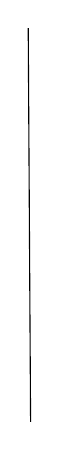
\begin{tikzpicture}\draw (0,0)--(.03,-5);\end{tikzpicture}}}}
\uline{Proposition} 11.11. Soi\deleted{\unsure{ent}}\handwritten{t} \deleted{$k$ un corps}, $G$ un \deleted{schéma en }groupe\deleted{s quasi-compact}\inserted{\handwritten{algébrique sur le}} \deleted{sur}\inserted{\handwritten{corps}} $k$. Les conditions suivantes sont équivalentes:

(i) $G$ est affine.

(ii) $G$ est quasi-affine.

(iii) On peut faire opérer $G$ fidèlement sur un\inserted{$k$-}schéma quasi-affine.

(iv) On peut faire opérer $G$ fidèlement sur un vectoriel sur $k$ (\unsure{pas} nécessairement de dimension finie).

(v) \deleted{(si $G$ est de type fini sur $k$),} $G$ est isomorphe à un sous-groupe fermé d'un groupe $\mathrm{GL}(n)_k$ .

\uline{Démonstration}. On a (i)$\handwritten{\Rightarrow}$(ii) trivialement, et (ii)$\handwritten{\Rightarrow}$(iii), car $G$ opère fidèlement sur lui-même par translations à gauche. On a (iii)$\handwritten{\Rightarrow}$(iv) car si $G$ opère \deleted{fidèlement sur $X$ quasi-affine sur $k$, alors il opère fidèlement sur l'envelopp\unsure{e} affine $X'=\operatorname{Spec}(\handwritten{\Gamma}($}\inserted{sur $X$ quasi-compact et quasi-séparé sur $k$, il opère aussi} sur le vectoriel $\handwritten{\Gamma}(X,\underline{O}_X)$, grâce au fait que la formation de $f_{\handwritten{*}}(\underline{O}_X)$ ($f:X\handwritten{\to}\operatorname{Spec}k$ le morphisme structural) commute à tout changement de base $S\handwritten{\to}\operatorname{Spec}k$ (EGA IV 1.7.12); donc il opère sur l'enveloppe affine $X'=\operatorname{Spec}(\handwritten{\Gamma}(X,\underline{O}_X))$, et le morphisme canonique $X\handwritten{\to}X'$ est évidemment compatible avec l'action de $G$; ceci dit, si $X$ est quasi-affine i.e. $X\handwritten{\to}X'$ est une immersion ouverte, et si $G$ opère fidèlement sur $X$, il opère fidèlement sur $X'$, ou ce qui revient au même, sur le vectoriel $V=\handwritten{\Gamma}(X,\underline{O}_X)$, ce qui prouve l'implication (iii)$\handwritten{\Rightarrow}$(iv).

\handwritten{S}upposons maintenant \deleted{que $G$ est de type fini, et}\inserted{\handwritten{(iv), i.e.}} que $G$ opère fidèlement sur le vectoriel $V$. Alors\handwritten{,}en vertu de 11.10\handwritten{,}$V$ est limite inductive de sous-es\handwritten{p}aces vectoriels $V_i$ de di\handwritten{m}ension finie, stables sous l'action de $G$. Si $K_i$ est le noyau de l'action induite de $G$ sur $V_i$ , i.e. de $G\handwritten{\to}\underline{\operatorname{Aut}}_{\inserted{\handwritten{V_i}}}\deleted{\unsure{(V_i)}}$, alors $K_i$ est un sous-schéma fermé de $G$, et l'hypothèse que $G$ opère fidèlement s'exprime aussitôt par le fait que \deleted{$K_{\unsure{1|i|l}}=e$ (\unsure{grou}} l'intersection des $K_i$ est le sous-groupe unité de $G$. Comme $G$ est noethé%
% archive sheet number: 48
\scanpage{50}%
\mspage{\handwritten{18}}%
rien, il s'ensuit que l'un des $K_i$ est déjà réduit au groupe unité, donc que $G\handwritten{\to}\underline{\operatorname{Aut}}_{\inserted{\handwritten{V_i}}}\deleted{\unsure{(V_i)}}$ est un monomorphisme. C'est donc une immersion fermée en vertu de (1.4.2), ce qui prouve que (iv)$\handwritten{\Rightarrow}$(v). Comme (v)$\handwritten{\Rightarrow}$(i) trivialement, cela prouve 11.11\deleted{\unsure{.}} pour $G$ de type fini.

\deleted{Prenons maintenant le cas général, où il reste à prouver que (iv)$\handwritten{\Rightarrow}$(i). Avec les notations de la démonstration précédente, soit $G_i$ le\inserted{plus petit} sous-groupe fermé de $\operatorname{Aut}(V_i)$ par lequel\inserted{peut} se factoriser $G\handwritten{\to}\underline{\operatorname{Aut}}_{\inserted{\handwritten{V_i}}}\deleted{\unsure{(V_i)}}$ \deleted{(existe} (un tel groupe existe, \deleted{puisque} comme intersection de tous ceux par lesquels se factorise $G\handwritten{\to}\deleted{\unsure{\operatorname{Aut}(V_i)}}\inserted{\underline{\operatorname{Aut}}_{V_i}}$). Si $V_j\handwritten{\supset}V_i$, on voit alors tout de suite que $G_j$ invarie $V_i$ , et que le morphisme correspondant $G_j\handwritten{\to}\underline{\operatorname{Aut}}_{V_i}$ se factorise par $G_i$ . De cette façon, les $G_i$ forment un système projectif de groupes affines sur $k$, et on a un morphisme naturel $G\handwritten{\longrightarrow}G'=\underset{\handwritten{\longleftarrow}}{\lim}G_i$ , où $G'$ est lui-même un groupe affine (EGA IV 8.2.3). L'hypothèse que $G$ opère \uline{fidèlement} sur $V$ s'exprime alors par\deleted{\unsure{r}} le fait que $G\handwritten{\to}G'$ est un monomorphisme. On a donc trouvé\handwritten{\makebox[0pt][l]{\raisebox{-.5ex}{\begin{tikzpicture}[x=.25cm,y=.25cm]\draw (0,-.5)--(.55,1);\end{tikzpicture}}}}un monomorphisme de $G$ dans un schéma affine, ce qui implique que le schéma quasi-compact\inserted{et séparé} $G$ est quasi-affine, i.e. que son faisceau structural est ample, en vertu de EGA IV 18.12.17 . En \handwritten{d}'autres termes, posant $H=\operatorname{Spec}\handwritten{\Gamma}(G,\underline{O}_G)$ , le morphisme canonique $G\handwritten{\to}H$ est une immersion ouverte. Notons maintenant que $H$ est de façon naturelle un schéma en groupes, et $G\handwritten{\to}H$ un homomorphisme de groupes, grâce à 11.2 . Cet homomorphisme est évidemment dominant, il reste à prouver que c'est un isomorphisme, ce qui résulte\deleted{\unsure{ra de}} du lemme suivant:}
\margin{\handwritten{\figure{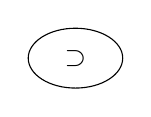
\begin{tikzpicture}
\draw (0,0) ellipse (.6 and .38);\node at (0,0) {$\supset$};
\end{tikzpicture}}}}

\deleted{\uline{Lemme} 11.11.1. Soient $\deleted{\unsure{G}}\handwritten{H}$ un schéma en groupes sur un corps\inserted{$k$}\handwritten{.} \deleted{$G$ un sous-} Alors tout sous-schéma en groupes ouvert\inserted{$G$} de $H$ est aussi fermé.}
\margin{\handwritten{\figure{\begin{tikzpicture}\draw (0,0)--(.03,-.8);\end{tikzpicture}}}}

\deleted{Il revient au même de dire que l'ensemble $H-G$ est ouvert, i.e. est un voisinage de chacun de ses points\deleted{\unsure{,}} $x$ . Or , toute extension de corps $k'/k$ définissant un morphisme $\operatorname{Spec}k'\handwritten{\to}\operatorname{Spec}k$ qui est universellement}
% archive sheet number: 49
